\documentclass[12pt,a4paper]{article}
\usepackage{ctex}
\usepackage{amsmath,amscd,amsbsy,amssymb,latexsym,url,bm,amsthm}
\usepackage{epsfig,graphicx,subfigure}
\usepackage{enumitem,balance}
\usepackage{wrapfig}
\usepackage{mathrsfs,euscript}
\usepackage[usenames]{xcolor}
\usepackage{hyperref}
\usepackage[vlined,ruled,linesnumbered]{algorithm2e}
\usepackage{array}
\hypersetup{colorlinks=true,linkcolor=black}

\newtheorem{theorem}{Theorem}
\newtheorem{lemma}[theorem]{Lemma}
\newtheorem{proposition}[theorem]{Proposition}
\newtheorem{corollary}[theorem]{Corollary}
\newtheorem{exercise}{Exercise}
\newtheorem*{solution}{Solution}
\newtheorem{definition}{Definition}
\theoremstyle{definition}

\renewcommand{\thefootnote}{\fnsymbol{footnote}}

\newcommand{\postscript}[2]
 {\setlength{\epsfxsize}{#2\hsize}
  \centerline{\epsfbox{#1}}}

\renewcommand{\baselinestretch}{1.0}

\setlength{\oddsidemargin}{-0.365in}
\setlength{\evensidemargin}{-0.365in}
\setlength{\topmargin}{-0.3in}
\setlength{\headheight}{0in}
\setlength{\headsep}{0in}
\setlength{\textheight}{10.1in}
\setlength{\textwidth}{7in}
\makeatletter \renewenvironment{proof}[1][Proof] {\par\pushQED{\qed}\normalfont\topsep6\p@\@plus6\p@\relax\trivlist\item[\hskip\labelsep\bfseries#1\@addpunct{.}]\ignorespaces}{\popQED\endtrivlist\@endpefalse} \makeatother
\makeatletter
\renewenvironment{solution}[1][Solution] {\par\pushQED{\qed}\normalfont\topsep6\p@\@plus6\p@\relax\trivlist\item[\hskip\labelsep\bfseries#1\@addpunct{.}]\ignorespaces}{\popQED\endtrivlist\@endpefalse} \makeatother

\begin{document}
\noindent

%========================================================================
\noindent\framebox[\linewidth]{\shortstack[c]{
\Large{\textbf{Lab08-Graph Exploration}}\vspace{1mm}\\
CS214-Algorithm and Complexity, Xiaofeng Gao \& Lei Wang, Spring 2021.}}
\begin{center}
\footnotesize{\color{red}$*$ If there is any problem, please contact TA Yihao Xie. }

\footnotesize{\color{blue}$*$ Name:\underline{Xin Xu}  \quad Student ID:\underline{519021910726} \quad Email: \underline{xuxin20010203@sjtu.edu.cn}}
\end{center}

\begin{enumerate}

	\item Given a graph $G = (V, E)$. Prove the following propositions.
	
	\begin{enumerate}
		\item Let $e$ be a maximum-weight edge on some cycle of connected graph $G=(V,E)$.
        Then there is a minimum spanning tree of $G$ that does not include $e$. Moreover, there is no minimum spanning tree of $G$ that includes $e$ if $e$ is the unique maximum-weight edge on the cycle. 
		\item Let $T$ and $T'$ are two different minimum spanning trees of $G$. Then $T'$ can be obtained from $T$ by repeatly substitute one edge in $T\backslash T'$ by one edge in $T'\backslash T$ and meanwhile the result after each subsitution is still a minimum spanning tree.
	\end{enumerate}

    \begin{proof}
        \begin{enumerate}
            \item For a spanning tree of a cycle with $n$ vertexes, it only needs $n-1$ edges. So, at least one edge must be quited. And for the Boruvka Algorithm, the maximum-weight edge $e$ will be omitted the first time(For the edge of the same weight, we would choose another one). So there is a minimum spanning tree contructed by Boruvka Algorithm does not include $e$.
            The next statement will be proved by contradiction. If $e$ is the unique maximum-weight edge on the cycle, and there is a minimum spanning tree includes $e$. Because of the definition of cycle, we can find another edge sticking to one of the vertexes of $e$ connects this vertex with other vertexes. So, we can just substitute this edgje with $e$ without the loss of optimum.
            And it's contracted to the definition of minimum spannign tree. So, the hypothesis is wrong, and the next statement is also true.
            \item Let $e\in E\backslash T$, and if we insert $e$ in the minimum spanning tree $T$, there will be a cycle $C$ in $e\bigcup T$. Find an $e$ satisfying $w(e)$ is not the maximum value of all edges' weight in $C$(if $e$ is of the maximum weight, $e$ is not unique). Substitute $e$ with the maximum-weight edge $m$, and this action doesn't hurt the optimum. Repeat this step until no such $e$ can be replaced.
        \end{enumerate}
    \end{proof}
	
    \item Let $G=(V,E)$ be a connected, undirected graph. Give an $O(|V|+|E|)$-time algorithm
    to compute a path in $G$ that traverses each edge in $E$ exactly once in each direction. Describe how you can find your way out of a maze if you are given a large supply of pennies.

    \begin{solution}
        The pseudocode is below:
      \\\begin{algorithm}[H]
            \KwIn{A connected, undirected graph $G=(V,E)$}
            \KwOut{A path in $G$ that traverses each edge in $E$ exactly once in each direction.}
            
            \BlankLine
            \caption{A path traverses every edge once}\label{Alg-travel path}

            $num\leftarrow 0$\;
            $start\leftarrow $ any $v\in V$\;
            \ForEach{ $v\in V$}{
                Compute the degree of $v$\;
                \If{$degree[v]$ is odd}{
                    $num\leftarrow num+1$\;
                    $start\leftarrow v$\;
                }
            }

            \If{$num\neq 0 $ and $num\neq 2$}{
                \Return{$error()$}\;
            }

            \ForEach{$v\in V$}{
                $VISITED[v]\leftarrow 0$\;
            }
            \ForEach{$e\in E$}{
                $VISITED[e]\leftarrow 0$\;
            }

            Start at $start$\;
            $path\leftarrow\varnothing $
            \For{$i\leftarrow 1$\KwTo $|E|$}{
                \If{find an $edge(start,u)\in E$ and $VISITED(u)=0$\;}{\;}
                \Else{find an $edge(start,u)\in E$ and $VISITED(edge(start,u))=0$\;}
                $path\leftarrow path\bigcup u$\;
                $start\leftarrow u$\;    
            }

            Output $path$\;

        \end{algorithm}

        To find a way out of a maze, I would first definite the vertexes and edges. Every block that is reachable in the maze is a vertex and only every two adjacent reachable blocks can be connected with edges. With these definitions, we can find the path use DFS Algorithm start at the beginning block. After DFS, examine whether the end block is in the path we just get. If it is, the path from beginning to the end is founded. If not, there is no such path.
    \end{solution}

    \item Consider the maze shown in Figure \ref{Fig-Maze}. The black blocks in the figure are blocks that can not be passed through. Suppose the block are explored in the order of right, down, left and up. That is, to go to the next block from $(X,Y)$, we always explore $(X,Y+1)$ first, and then $(X+1,Y)$,$(X,Y-1)$ and$(X-1,Y)$ at last. Answer the following subquestions:
    \begin{enumerate}
        \item Give the sequence of the blocks explored by using DFS to find a path from the "start" to the "finish".
        \item Give the sequence of the blocks explored by using BFS to find the \underline{shortest} path from the "start" to the "finish".
        \item Consider a maze with a larger size. Discuss which of BFS and DFS will be used to find one path and which will be used to find the shortest path from the start block to the finish block.
    \end{enumerate}
    
    \begin{figure}[!htbp]
	\centering
	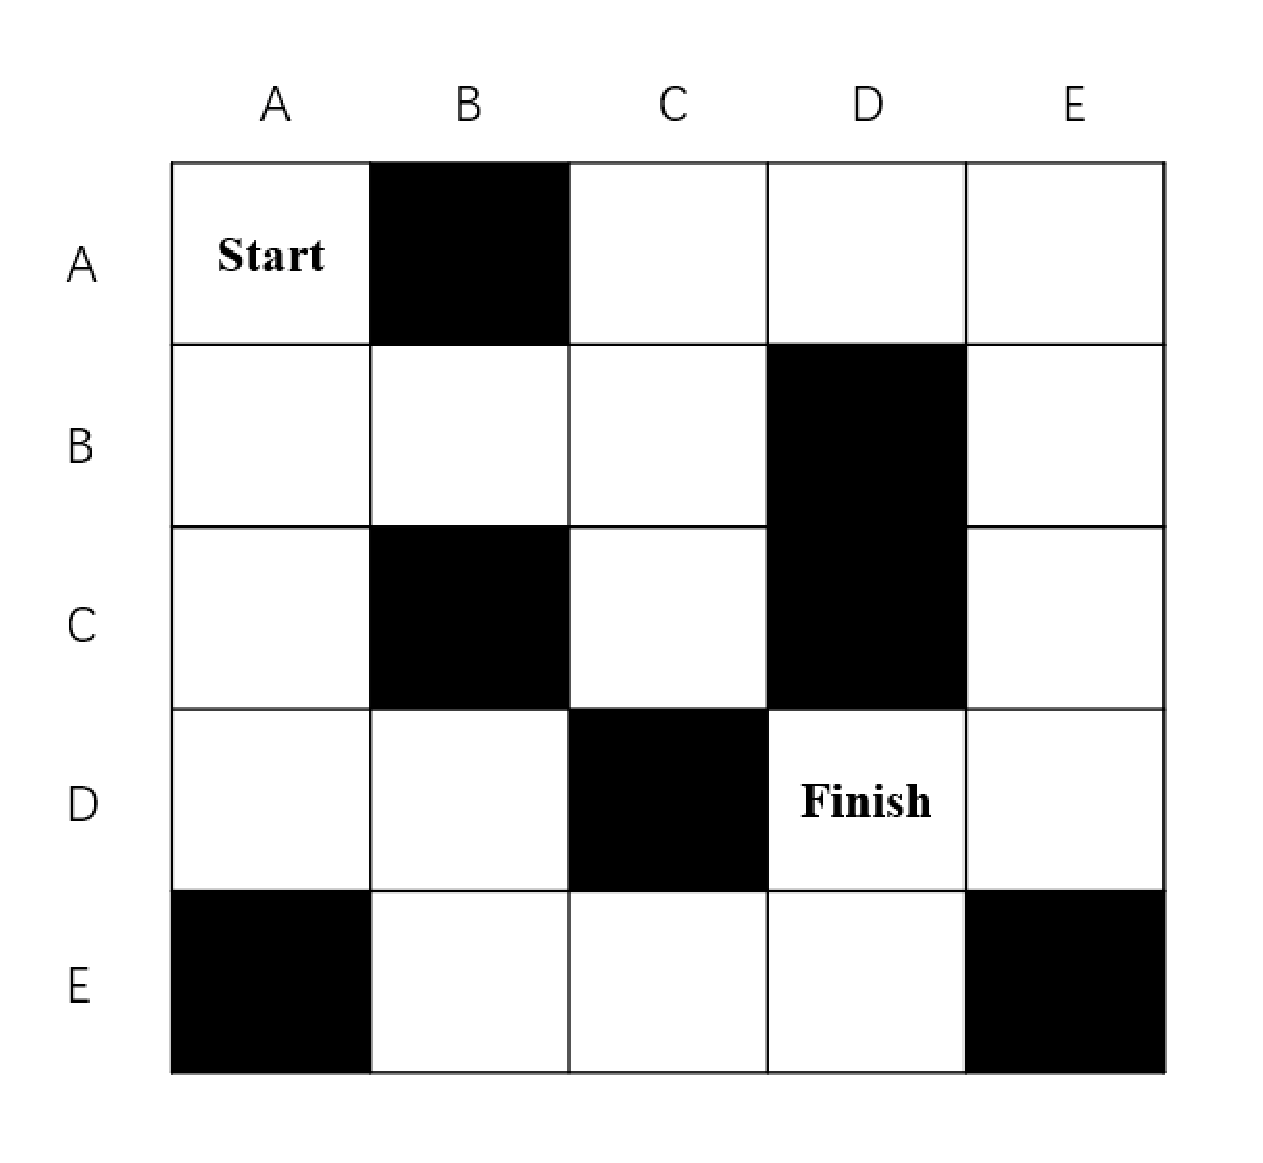
\includegraphics[width=0.5\textwidth]{Fig-Maze.pdf}
	\caption{An example of making room for one new element in the set of arrays.}
	\label{Fig-Maze}
	\end{figure}

    \begin{solution}
        \begin{enumerate}
            \item The path is $(A,A)\rightarrow (B,A)\rightarrow (B,B)\rightarrow (B,C)\rightarrow (A,C)\rightarrow (A,D)\rightarrow (A,E)\rightarrow (B,E)\rightarrow (C,E)\rightarrow (D,E)\rightarrow (D,D)$.
            \item The path is $(A,A)\rightarrow (B,A)\rightarrow (C,A)\rightarrow (D,A)\rightarrow (D,B)\rightarrow (E,B)\rightarrow (E,C)\rightarrow (E,D)\rightarrow (D,D)$.
            \item DFS and BFS both can be used to find one path but DFS is more efficient. And BFS is more suitable to find the shortest path from the start block to the finish block.
        \end{enumerate}
    \end{solution}
	
	\item Given a directed graph $G$, whose vertices and edges information are introduced in data file "SCC.in". Please find its number of Strongly Connected Components with respect to the following subquestions.
    
    \begin{enumerate}
    	\item Read the code and explanations of the provided C/C++ source code "SCC.cpp", and try to complete this implementation.
    	\item Visualize the above selected Strongly Connected Components for this graph $G$. Use the $Gephi$ or other software you preferred to draw the graph. {\color{blue}(If you feel that the data provided in ``SCC.in'' is not beautiful, you can also generate your own data with more vertices and edges than $G$ and draw an additional graph. Notice that results of your visualization will be taken into the consideration of Best Lab.)}
    \end{enumerate}	

    \begin{solution}
        \begin{enumerate}
            \item The implementation is in the .cpp file. And the output in .out file is 202.
            \item The picture is in the last page.
            \begin{figure}[htbp]
                \centering
                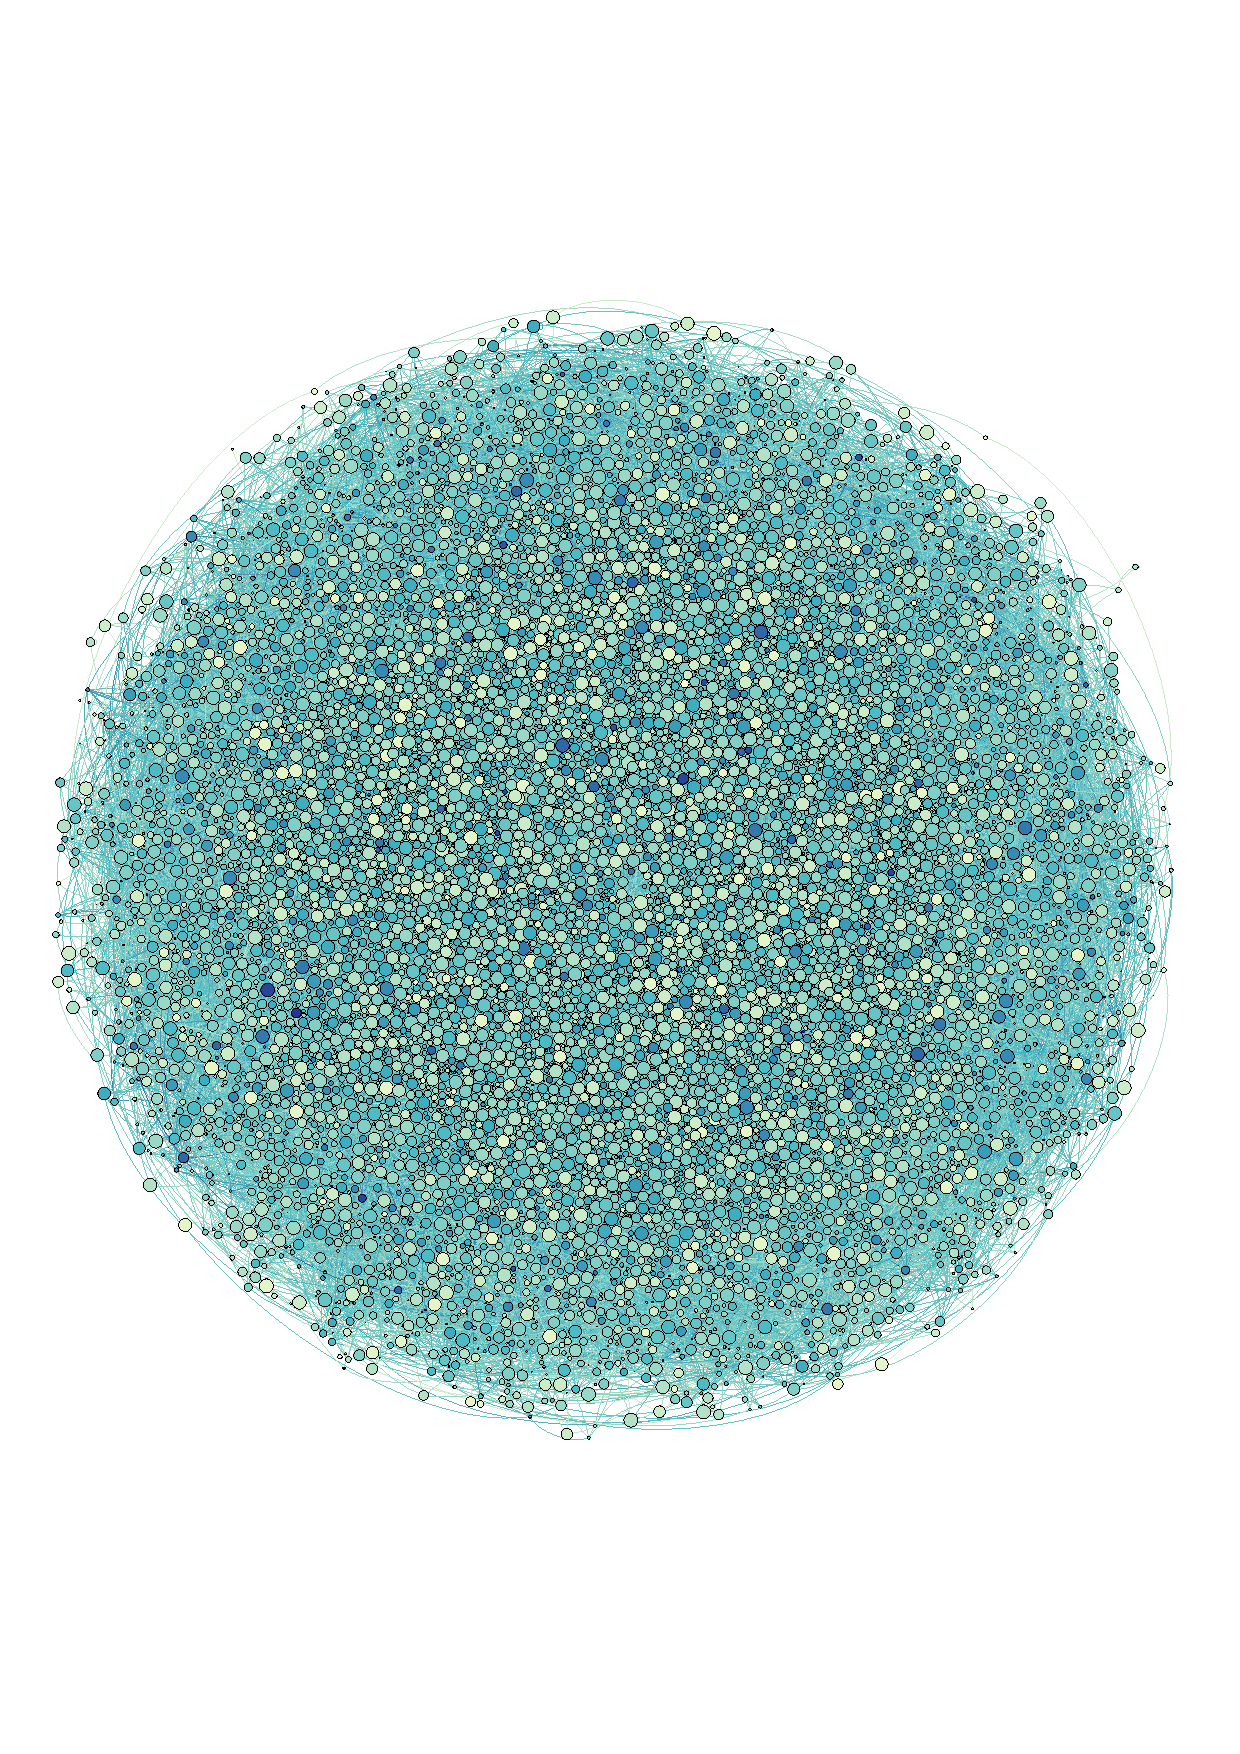
\includegraphics[width=0.4\textwidth]{SCC.pdf}
                \caption{Visualization of directed graph}\label{SCC}
            \end{figure}

        \end{enumerate}
    \end{solution}

\end{enumerate}



\textbf{Remark:} Please include your .pdf, .tex, .cpp files for uploading with standard file names.
\newpage


%========================================================================
\end{document}